%TeX

\section{Reversing the MBR}

\subsection{RE400 what?}

\begin{frame}{RE400 what?\ldots}
    \begin{columns}
        \column{0.5\textwidth}
	        \begin{itemize}
                \item Challenge worth 400 points
                \item Reverse Engineering category
                \item We get some hints right away\ldots
                \begin{itemize}
                	\item This is an MBR
                	\item \ldots from an x86 system
        	    \end{itemize}
            \end{itemize}
        \column{0.5\textwidth}
                {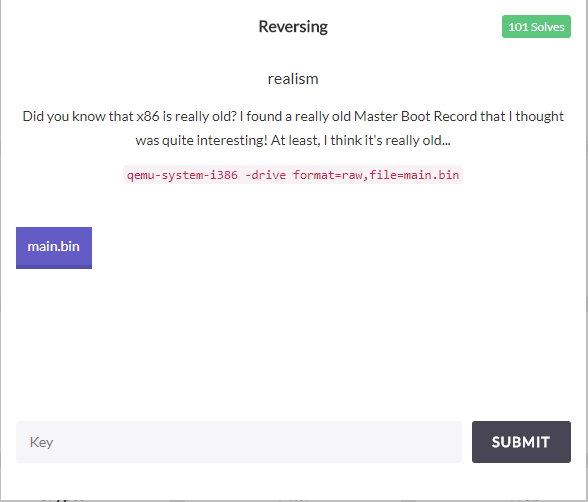
\includegraphics[width=\textwidth]{re400}}
    \end{columns}
\end{frame}

\begin{frame}{A place to start\ldots}
    \begin{columns}
        \column{0.5\textwidth}
	        \begin{itemize}
                \item<1-> Wikipedia, of course!
		        \begin{itemize}
    	            \item<2-> 512 bytes
        	        \item<2-> MBR signature: 55 AA
            	    \item<2-> "expected to contain real mode machine language instructions"
                	\item<2-> little-endian
                	\item<2-> loads at 0000:7C00
	            \end{itemize}                	
            \end{itemize}
        \column{0.5\textwidth}
                {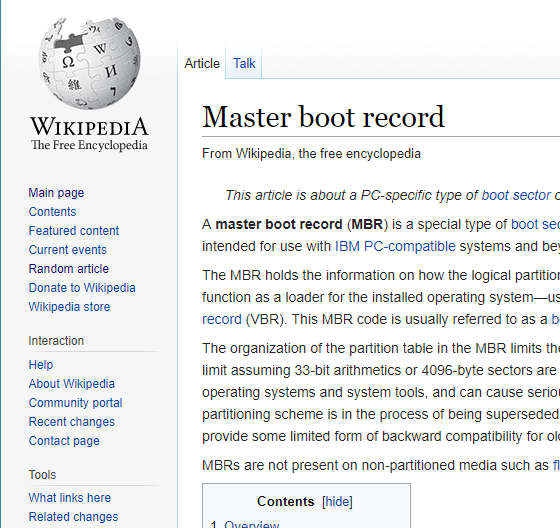
\includegraphics[width=\textwidth]{wikimbr}}
    \end{columns}
\end{frame}

\subsection{Tools}

\begin{frame}{Tool Time!\ldots}
    \framesubtitle{qemu (gift wrapped)}
    \begin{columns}
        \column{0.5\textwidth}
            \only<1> {
              	\begin{itemize}
             		\item -s (gdb)
                	\item -S (suspend)
        	       	\item -vnc:1
	            \end{itemize}
            }
            \only<2> {
             	\begin{itemize}
            		\item QEMU/Monitor
              		\begin{itemize}
	    	        	\item info registers
    	    	       	\item system reset
    	    	    \end{itemize}
        	    \end{itemize}
        	}
        \column{0.5\textwidth}
            \only<1>{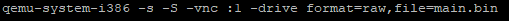
\includegraphics[width=\textwidth]{launch-qemu}\newline\newline
            		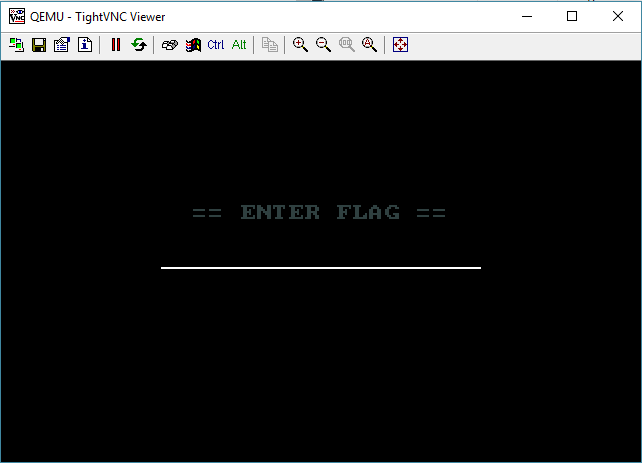
\includegraphics[width=\textwidth]{qemu-vnc}
			}
            \only<2>{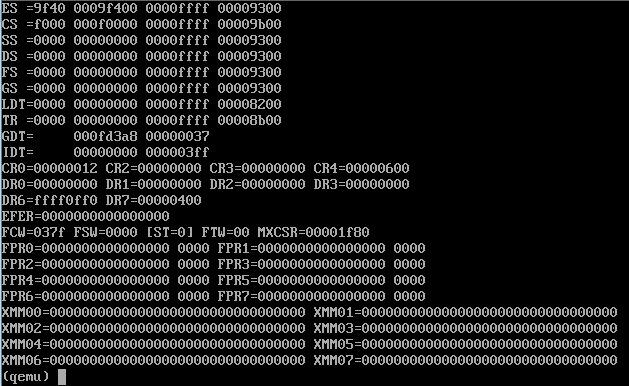
\includegraphics[width=\textwidth]{qemu-info-registers-1}}
    \end{columns}
\end{frame}

\begin{frame}{Tool Time!\ldots}
    \framesubtitle{gdb}
    \begin{columns}
        \column{0.5\textwidth}
                \begin{itemize}
                	\only<1>{
						\item target remote localhost:1234
						\item set architecture i8086
							(bootloaders are 16 bit, right?)
						\item display/i \$pc - print program counter
						\item br *0xADDR - set breakpoint
						\item si - run one instruction
						\item c - continue
					}
					\only<2->{
						\item info reg
						\uncover<3->{\item info frame}
						\uncover<4->{\item x /CT 0xADDR - display C units of T type from ADDR
									\item set \{int\}0xADDR = 42
									\item set \{char[4]\} 0xADDR = "AAA"
						}
					}
				\end{itemize}
		\column{0.5\textwidth}
				\only<1>{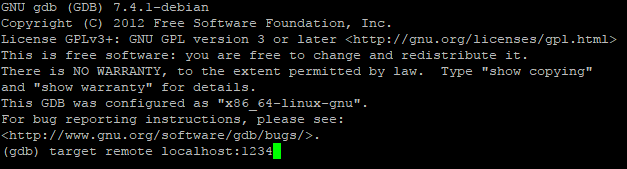
\includegraphics[width=\textwidth]{launch-gdb}\newline\newline
						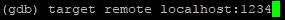
\includegraphics[width=\textwidth]{gdb-target}}
				\only<2>{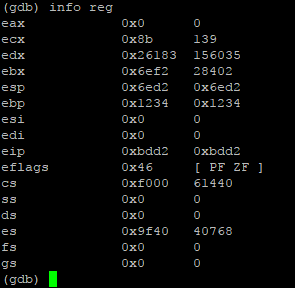
\includegraphics[width=\textwidth]{gdb-info-reg-1}}
				\only<3>{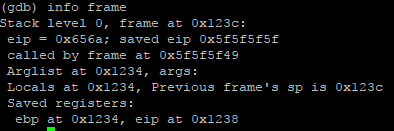
\includegraphics[width=\textwidth]{gdb-info-frame}}
				\only<4-5>{
					\uncover<4->{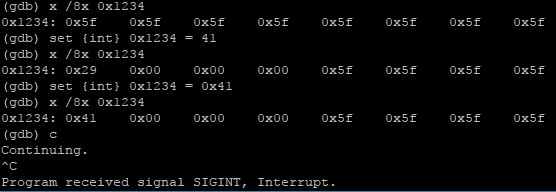
\includegraphics[width=\textwidth]{gdb-x-set-1}}
					\uncover<5->{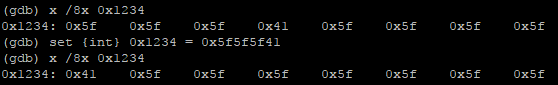
\includegraphics[width=\textwidth]{gdb-x-set-2}}
				}
				\only<6>{
					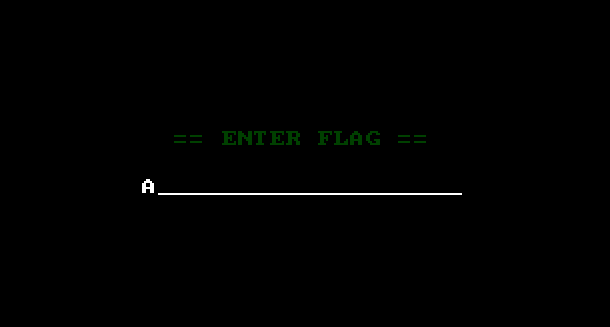
\includegraphics[width=\textwidth]{after-set}
				}
	\end{columns}
\end{frame}

\begin{frame}{Tool Time!\ldots}
    \framesubtitle{IDA}
    \begin{columns}
        \column{0.5\textwidth}
            \begin{itemize}
                \item Rebase
                \uncover<2->{
                	\item Common ASM
                	\only<2>{
         		       	\begin{itemize}
     	    	       		\item int
     		           		\item mov
             		   		\item inc, dec
                			\item and, or, not, xor...
                			\item cmp
	                		\item jmp, jz, jge, jle...
	                	\end{itemize}
	                }
	            }
	            \uncover<3->{
	            	\item Registers
	            	\only<3>{
         		       	\begin{itemize}
     	    	       		\item E AX - Accumulator
     		           		\item E CX - Counter
             		   		\item E DX - Data
                			\item E BX - Base
                			\item E SP - Stack pointer
	                		\item E BP - Stack base pointer
	                		\item E SI - Source
	                		\item E DI - Destination
	                	\end{itemize}
	                }
	            }
			\end{itemize}
		\column{0.5\textwidth}
			\only<1>{
				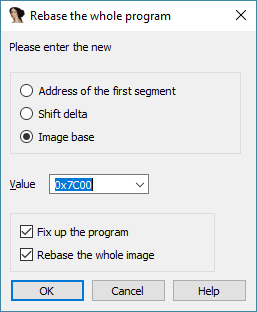
\includegraphics[width=\textwidth]{rebase}
			}
			\only<2->{
				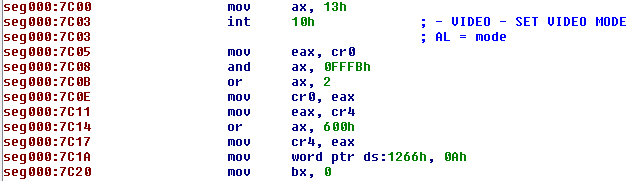
\includegraphics[width=\textwidth]{ida-first}
			}
	\end{columns}
\end{frame}

\subsection{Disassembly and reversing}

\begin{frame}{Disassembly\ldots}
    \begin{columns}
        \column{0.5\textwidth}
            \begin{itemize}
                \item Look for hints
                \begin{itemize}
                	\uncover<2->{
         	 	      	\item Loops
	     	       }
	          	  \uncover<3->{
	            		\item Comparisons
	            	}
	            	\uncover<4->{
	            		\item Unknowns
		            }
				\end{itemize}
			\end{itemize}
		\column{0.5\textwidth}
			\only<2>{
				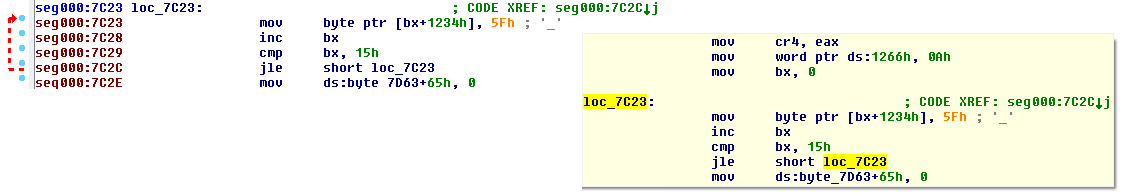
\includegraphics[width=\textwidth]{loop}
			}
			\only<3>{
				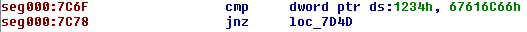
\includegraphics[width=\textwidth]{cmp1}
			}
			\only<4>{
				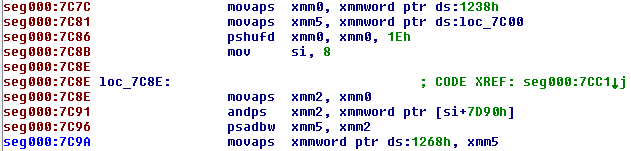
\includegraphics[width=\textwidth]{sse}
			}
	\end{columns}
\end{frame}

\begin{frame}{Putting it all together\ldots}
    \begin{columns}
        \column{0.5\textwidth}
            \begin{itemize}
                \item We know that 0x7C6F compares user input to "flag"
                \uncover<2->{\item There's a bunch of complicated instructions right after that cmp}
	     	    \uncover<3->{\item We can use gdb and qemu/monitor to see what's happening...}
	     	    \uncover<4->{\item Now we just have to work backwards from there.}
			\end{itemize}
		\column{0.5\textwidth}
			\only<1>{
				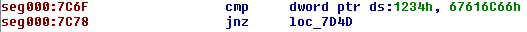
\includegraphics[width=\textwidth]{cmp1}
			}
			\only<2>{
				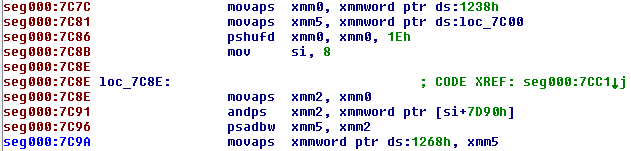
\includegraphics[width=\textwidth]{sse}
			}
			\only<3->{
				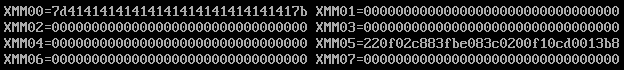
\includegraphics[width=\textwidth]{reg1}
			}
			\uncover<4>{
				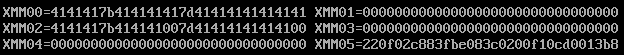
\includegraphics[width=\textwidth]{reg2}
			}
	\end{columns}
\end{frame}

\begin{frame}{Other useful tools\ldots that I didn't know about}
	\begin{itemize}
		\item Binary Ninja
 		\item pwndbg
 		\item Radare
 	\end{itemize}
\end{frame}
